\documentclass{beamer}
% basic packages
\usepackage{xcolor}
\usepackage[utf8]{inputenc}

\usepackage{amsmath}
\usepackage{graphicx}
\usepackage{lmodern}
\usepackage[T1]{fontenc}
% tikz libraries
\usepackage{tikz}
\usetikzlibrary{decorations,arrows,shapes,automata,shadows}
\usetikzlibrary{decorations.markings}
%colors
\definecolor{plantfill}{rgb}{0.960784,   0.850980,   0.039216}
\definecolor{plantline}{rgb}{0.77647,   0.53725,   0.00000}
\definecolor{superfill}{rgb}{0.54510,   0.88235,   0.15686}
\definecolor{superline}{rgb}{0.227451,   0.486275 ,  0.054902}
\definecolor{specfill}{rgb}{0.42353,   0.43922,   0.72157}
\definecolor{specline}{rgb}{0.00000,   0.05098,   0.36471}
\definecolor{uobsb}{rgb}{0.10980,   0.30196,   0.94510 } 
\definecolor{uobsg}{rgb}{0.035294,   0.533333,   0.458824 } 
\definecolor{auto_color}{rgb}{0,0,0}
\definecolor{bg_color}{rgb}{ 0.98823529,  0.98823529,  0.58039216}
\definecolor{skyfill}{rgb}{  0.50196,   0.70196,   1.00000}
\definecolor{skyline}{rgb}{0.00000,   0.23922,   0.75294 }
\definecolor{yellowfill}{rgb}{1.00000,   0.90196,   0.50196}
\definecolor{yellowline}{rgb}{1.00000,   0.4,   0}

% beamer data
\author{LCA--Lab. de Controle e Automac\~ao}
\title{DESLab Software Package}
\usetheme{Madrid}
\usecolortheme{seagull}
\setbeamercolor{normal text}{bg=bg_color!30}
\usefonttheme{professionalfonts}

% special arrow definition
\newdimen\dima
\newdimen\dimb

\pgfarrowsdeclare{deslab}{deslab}
{
  \dima=0.05pt%
  \advance\dima by.3\pgflinewidth%
  \dimb=6\dima\advance\dimb by.5\pgflinewidth%
  \pgfarrowsleftextend{+-\dimb}
  \dimb=2\dima\advance\dimb by0.5\pgflinewidth%
  \pgfarrowsrightextend{+\dimb}
}
{
  \dima=0.05pt%
  \advance\dima by.3\pgflinewidth%
  \pgfsetdash{}{-0pt}
  \pgfsetroundjoin
  \pgfpathmoveto{\pgfqpoint{2\dima}{0\dima}}
  \pgfpathcurveto
  {\pgfqpoint{-.5\dima}{.5\dima}}
  {\pgfqpoint{-3\dima}{1.5\dima}}
  {\pgfqpoint{-6\dima}{3.25\dima}}
  \pgfpathcurveto
  {\pgfqpoint{-3\dima}{1\dima}}
  {\pgfqpoint{-3\dima}{-1\dima}}
  {\pgfqpoint{-6\dima}{-3.25\dima}}
  \pgfpathcurveto
  {\pgfqpoint{-3\dima}{-1.5\dima}}
  {\pgfqpoint{-.5\dima}{-.5\dima}}
  {\pgfqpoint{2\dima}{0\dima}}
  \pgfpathclose
  \pgfusepathqfillstroke
}

\pgfarrowsdeclare{deslab'}{deslab'}
{
  \dima=0.05pt%
  \advance\dima by.3\pgflinewidth%
  \pgfarrowsleftextend{+-4\dima}
  \pgfarrowsrightextend{+6\dima}
}
{
  \dima=0.05pt%
  \advance\dima by.3\pgflinewidth%
  \pgfpathmoveto{\pgfqpoint{6\dima}{0\dima}}
  \pgfpathcurveto
  {\pgfqpoint{3.5\dima}{.5\dima}}
  {\pgfqpoint{-1\dima}{1.5\dima}}
  {\pgfqpoint{-4\dima}{3.75\dima}}
  \pgfpathcurveto
  {\pgfqpoint{-1.5\dima}{1\dima}}
  {\pgfqpoint{-1.5\dima}{-1\dima}}
  {\pgfqpoint{-4\dima}{-3.75\dima}}
  \pgfpathcurveto
  {\pgfqpoint{-1\dima}{-1.5\dima}}
  {\pgfqpoint{3.5\dima}{-.5\dima}}
  {\pgfqpoint{6\dima}{0\dima}}
  \pgfusepathqfill
}

\pgfarrowsdeclare{init}{init}
{
  \dima=0.05pt%
  \advance\dima by.25\pgflinewidth%
  \dimb=5.5\dima\advance\dimb by.5\pgflinewidth%
  \pgfarrowsleftextend{+-\dimb}
  \dimb=.5\dima\advance\dimb by0.707\pgflinewidth%
  \pgfarrowsrightextend{+\dimb}
}
{
  \dima=0.05pt%
  \advance\dima by.25\pgflinewidth%
  \pgfsetdash{}{+0pt}
  \pgfsetmiterjoin
  \pgfpathmoveto{\pgfqpoint{-5.5\dima}{-6\dima}}
  \pgfpathlineto{\pgfqpoint{0.5\dima}{0\dima}}
  \pgfpathlineto{\pgfqpoint{-5.5\dima}{6\dima}}
  \pgfpathclose
  \pgfusepathqfillstroke
}

\pgfarrowsdeclare{init'}{init'}
{
  \dima=0.05pt%
  \advance\dima by.25\pgflinewidth%
  \pgfarrowsleftextend{+-.5\pgflinewidth}
  \dimb=6\dima\advance\dimb by0.707\pgflinewidth%
  \pgfarrowsrightextend{+\dimb}
}
{
  \dima=0.05pt%
  \advance\dima by.25\pgflinewidth%
  \pgfsetdash{}{+0pt}
  \pgfsetmiterjoin
  \pgfpathmoveto{\pgfqpoint{0\dima}{-6\dima}}
  \pgfpathlineto{\pgfqpoint{6\dima}{0\dima}}
  \pgfpathlineto{\pgfqpoint{0\dima}{6\dima}}
  \pgfpathclose
  \pgfusepathqstroke
}



\begin{document}
%font selection
\fontsize{1pt}{1pt}
\selectfont
\tikzset{obs_edge arrow/.style={->, >=deslab, line width =0.075pt}}
\tikzset{accepting/.style={double distance=0.1pt}}

        
\tikzset{unobs_edge arrow/.style={->, >=deslab, dash pattern=on 0.1pt off 0.15pt, draw = uobsg,
line width =0.075pt}}

\tikzset{every initial by arrow/.style=
{>=init, initial distance=1.7pt,line width=0.125pt, initial where=, fill =yellow!60, draw =green!30!black, initial text={}}}

\tikzset{every state/.style={draw= plantline!85, fill= plantfill!76, line width = 0.1, inner sep= 0.25pt, minimum size=0pt, circle,}}
        
\begin{frame}       
\frametitle{\textcolor{auto_color}{\textcolor{white}{\framebox{Fig. \; 0.0 }\quad} $G_1$}}
\begin{center}
\resizebox{100mm}{!}{
\begin{tikzpicture}
%%
\node (s1) at (2.70pt,1.80pt) [draw,ellipse,state,initial] {$q_1$};
  \node (s0) at (12.40pt,1.80pt) [draw,ellipse,state] {$q_2$};
  \node (s2) at (22.10pt,1.80pt) [draw,ellipse,state] {$q_3$};
  \draw [,obs_edge arrow] (s1) ..controls (6.43pt,1.80pt) and (7.60pt,1.80pt)  .. (s0);
  \definecolor{strokecol}{rgb}{0.0,0.0,0.0};
  \pgfsetstrokecolor{strokecol}
  \draw (7.55pt,2.55pt) node {$b_1$};
  \draw [,obs_edge arrow] (s0) ..controls (16.13pt,1.80pt) and (17.30pt,1.80pt)  .. (s2);
  \draw (17.25pt,2.55pt) node {$b_1$};
  \draw [,obs_edge arrow] (s2) ..controls (21.08pt,4.51pt) and (21.37pt,5.40pt)  .. (22.10pt,5.40pt) .. controls (22.56pt,5.40pt) and (22.84pt,5.05pt)  .. (s2);
  \draw (22.10pt,6.15pt) node {$a_1$};
%

\end{tikzpicture}} 
 \end{center} 
 \end{frame}        
\tikzset{unobs_edge arrow/.style={->, >=deslab, dash pattern=on 0.1pt off 0.15pt, draw = uobsg,
line width =0.075pt}}

\tikzset{every initial by arrow/.style=
{>=init, initial distance=1.7pt,line width=0.125pt, initial where=, fill =yellow!60, draw =green!30!black, initial text={}}}

\tikzset{every state/.style={draw= plantline!85, fill= plantfill!76, line width = 0.1, inner sep= 0.25pt, minimum size=0pt, circle,}}
        
\begin{frame}       
\frametitle{\textcolor{auto_color}{\textcolor{white}{\framebox{Fig. \; 0.1 }\quad} $G_1$}}
\begin{center}
\resizebox{100mm}{!}{
\begin{tikzpicture}
%%
\node (s0) at (2.70pt,1.80pt) [draw,ellipse,state] {$q_2$};
  \node (s2) at (12.40pt,1.80pt) [draw,ellipse,state] {$q_3$};
  \draw [,obs_edge arrow] (s0) ..controls (6.43pt,1.80pt) and (7.60pt,1.80pt)  .. (s2);
  \definecolor{strokecol}{rgb}{0.0,0.0,0.0};
  \pgfsetstrokecolor{strokecol}
  \draw (7.55pt,2.55pt) node {$b_1$};
  \draw [,obs_edge arrow] (s2) ..controls (11.38pt,4.51pt) and (11.67pt,5.40pt)  .. (12.40pt,5.40pt) .. controls (12.86pt,5.40pt) and (13.14pt,5.05pt)  .. (s2);
  \draw (12.40pt,6.15pt) node {$a_1$};
%

\end{tikzpicture}} 
 \end{center} 
 \end{frame}        
\tikzset{unobs_edge arrow/.style={->, >=deslab, dash pattern=on 0.1pt off 0.15pt, draw = uobsg,
line width =0.075pt}}

\tikzset{every initial by arrow/.style=
{>=init, initial distance=1.7pt,line width=0.125pt, initial where=, fill =yellow!60, draw =green!30!black, initial text={}}}

\tikzset{every state/.style={draw= plantline!85, fill= plantfill!76, line width = 0.1, inner sep= 0.25pt, minimum size=0pt, circle,}}
        
\begin{frame}       
\frametitle{\textcolor{auto_color}{\textcolor{white}{\framebox{Fig. \; 0.2 }\quad} Empty Automaton}}
\begin{center}
\resizebox{50mm}{!}{
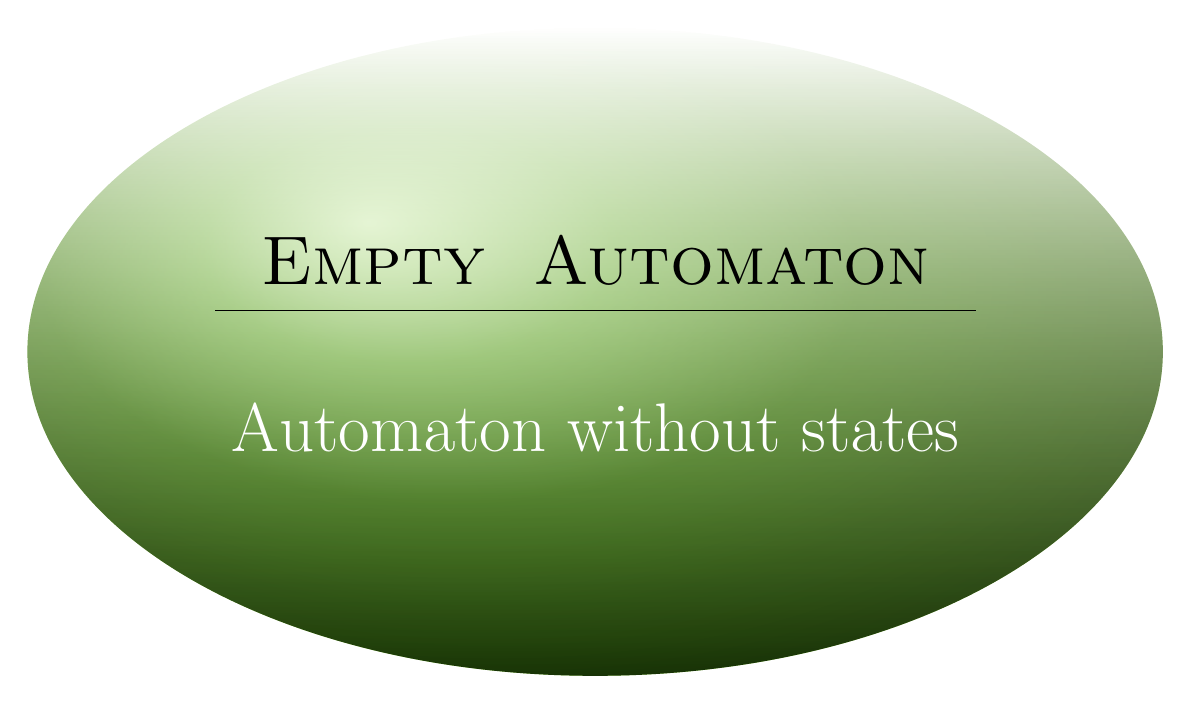
\begin{tikzpicture}
\tikzset{every initial by arrow/.style=
{>=initarrow,initial distance=50pt, draw=specline, line width=4pt, initial where= above, initial text={}}}
\fontsize{30pt}{30pt}
\selectfont
\node (s1) at (2,2) [ellipse,line width=1pt, ball color=superline, path fading=north, fill=superfill!70 ] {
\begin{tabular}{c}
\\
{\textsc{Empty }}
{\textsc{Automaton}}\\
\hline
\\
\textcolor{white}{ Automaton without states}\\
\\
\end{tabular}};

\end{tikzpicture}} 
 \end{center} 
 \end{frame}\end{document}